\chapter{Literature Review and Theoretical Foundations}

The reconstruction of three-dimensional environments from two-dimensional observations has been studied since the early 1980s, and its evolution can be read as a sequence of paradigm shifts. First came the geometric era, in which reconstruction was a purely numerical exercise on matched pixel pairs. Then came the implicit-neural era, which replaced discrete geometry with continuous functions parametrised by deep networks. Finally we arrive at the explicit radiance-field era, which reinstated explicit primitives while preserving differentiability. The method developed in this thesis lives at the very end of this chain and, additionally, at the intersection with a fourth, currently active front, the extension of radiance-field methods to temporally varying scenes. This chapter reviews the four fronts in turn, giving extra weight to 3D Gaussian Splatting (the immediate ancestor of the proposed method) and to the small but growing body of work on four-dimensional radiance fields (the direct comparison baseline), and closes with the formal mathematical background that Chapter~3 will build upon.

\section{Geometric Foundations: Structure from Motion}

Before the rise of deep learning, three-dimensional reconstruction was dominated by photogrammetry and geometric computer vision. These methods rely on triangulation, if a single physical point is observed in at least two cameras with known relative pose, its 3D location can be recovered as the intersection of the corresponding viewing rays. The central technical problem is therefore not triangulation itself but the joint estimation of the unknown camera poses and the correspondences that feed it.

\subsection{Early Structure-from-Motion}

The theoretical groundwork for modern multi-view reconstruction was laid by Longuet-Higgins \cite{Longuet-Higgins1981}, who introduced the 8-point algorithm, a closed-form recovery of the essential matrix from eight or more point correspondences between two calibrated views. The algorithm proved that the relative geometry of a pair of cameras could be determined linearly, without any iterative optimisation, from a small set of pixel correspondences. It remains the textbook method for the two-view initialisation problem, and it is still the mechanism used by COLMAP to bootstrap its incremental reconstruction when no initial camera pose is available.

Building on this two-view result, Tomasi and Kanade \cite{Tomasi1992} introduced the Factorisation Method. Their observation was that, under an orthographic projection model, the measurement matrix $W \in \mathbb{R}^{2F \times P}$ stacking the tracked image coordinates of $P$ feature points over $F$ frames has rank at most $3$. A Singular Value Decomposition of $W$ therefore factorises jointly the camera motion $M \in \mathbb{R}^{2F \times 3}$ and the shape $S \in \mathbb{R}^{3 \times P}$:
\begin{equation}
    W = M S, \qquad \text{rank}(W) = 3 \text{ (orthographic projection)}.
\end{equation}
The factorisation method is historically important because it was the first algorithm to recover motion and shape \emph{simultaneously} from a rank constraint, an idea that reappears in different form in essentially every modern SfM pipeline.

\subsection{Scaling Up: Photo Tourism and Bundler}

Early SfM systems worked on small, curated image sets. Snavely et al.~\cite{10.1145/1179352.1141964} demonstrated for the first time that SfM could be scaled to heterogeneous collections of thousands of consumer photographs. Their Photo Tourism system, later released as Bundler, exploited the viewpoint invariance of the SIFT descriptor \cite{lowe1999sift} to build robust pairwise matches across widely different viewpoints and then recovered the full camera set through incremental bundle adjustment. Bundler was the first system to cross the threshold from a theoretical idea to a tool usable on unconstrained imagery. It was a groundwork that directly influenced the design of every incremental SfM pipeline since, including COLMAP. The inputs and output of Bundler can be seen on Figure \ref{fig:bundler}.

Bundler produced only a sparse point cloud. To densify the reconstruction, Furukawa and Ponce~\cite{Furukawa2010-ge} introduced PMVS (Patch-based Multi-View Stereo), which represents surfaces as collections of small, oriented rectangular patches rather than individual pixels or voxels. PMVS is notable in the context of this thesis because it clearly illustrates a fundamental trade-off that reappears in Gaussian Splatting, explicit patch-based representations offer better scaling and better locality than dense voxel grids, at the cost of a more complex growth-and-filter optimisation.

\begin{figure}[!ht]
    \begin{center}
        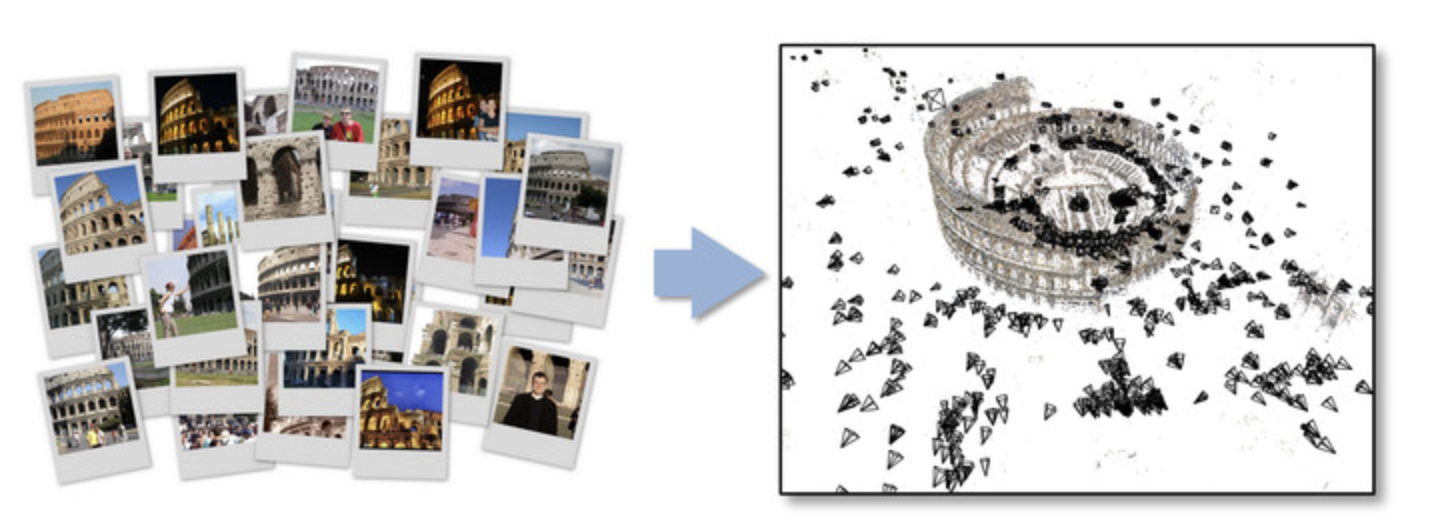
\includegraphics[width=1.0\linewidth]{res/02_literature/bundler.png}
    \end{center}
    \caption{Photo taken from the Snavely et al.~\cite{10.1145/1179352.1141964} showing how Bundler transforms set of photos to sparse 3D cloud point, which can be navigated and explored in a 3D rendering software.}
    \label{fig:bundler}
\end{figure}

\subsection{The Current Geometric Gold Standard: COLMAP}

Sch\"{o}nberger and Frahm \cite{schoenberger2016sfm} revisited the incremental SfM pipeline with a particular focus on robustness and completeness. Their system, COLMAP, introduced three important improvements over Bundler:
\begin{itemize}
    \item More rigorous ''next best view'' selection strategy that prefers images contributing the most stable geometric information to the existing reconstruction.

    \item Frequent global bundle adjustment with outlier filtering to counteract drift.

    \item Mature feature-matching stage that gracefully degrades from exhaustive matching to vocabulary-tree-based matching as the image count grows.
\end{itemize}

COLMAP remains the de facto standard initialisation stage for every modern radiance-field method: NeRF, Instant-NGP, and 3DGS all consume COLMAP output natively. This is also its role in the present thesis: COLMAP produces the sparse point cloud and the camera extrinsics that seed the Gaussian Splatting optimiser. Its limitation, however, is structural: its output is a discrete point cloud, and no matter how dense, a point cloud cannot model continuous surfaces or view-dependent shading without substantial post-processing. Closing that gap is precisely what radiance-field methods exist for.

\section{The Neural Shift: Implicit Representations}

By the mid-2010s, deep learning was outperforming hand-engineered features in image classification, but 3D reconstruction remained essentially geometric. Early deep-learning attempts treated 3D reconstruction as voxel prediction, as in 3D-R2N2 \cite{choy2016}. These approaches were limited by the cubic memory complexity of voxel grids: at $32^3$ resolution they could represent shape only coarsely, and scaling to resolutions sufficient for indoor scenes was infeasible. The implicit-neural paradigm that followed sidestepped the problem by replacing the discrete grid with a continuous function.

\begin{figure}[!ht]
    \begin{center}
        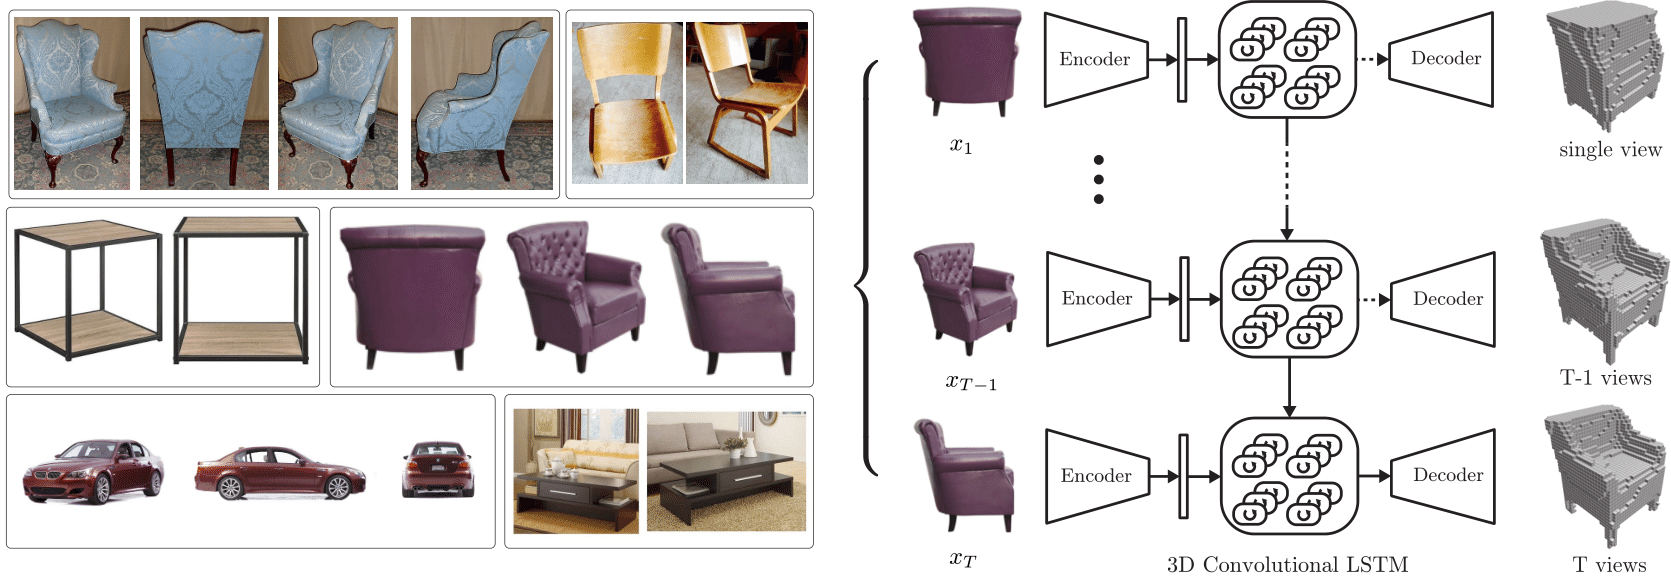
\includegraphics[width=1.0\linewidth]{res/02_literature/3d-r2n2.png}
    \end{center}
    \caption{Pipeline showing how 3D-R2N2 \cite{choy2016} transforms a set of images to 3D voxel representation.}
    \label{fig:3d-r2n2}
\end{figure}

\subsection{Neural Radiance Fields (NeRF)}

Mildenhall et al.~\cite{mildenhall2020} proposed Neural Radiance Fields, which represent a scene as a continuous function $F_\theta$ implemented by a Multilayer Perceptron (MLP):
\begin{equation}
    F_\theta : (\mathbf{x}, \mathbf{d}) \in \mathbb{R}^3 \times \mathbb{S}^2 \; \mapsto \; (\mathbf{c}, \sigma) \in \mathbb{R}^3 \times \mathbb{R}_{\geq 0},
\end{equation}
mapping a spatial location $\mathbf{x}$ and a viewing direction $\mathbf{d}$ to a view-dependent colour $\mathbf{c}$ and a view-independent volumetric density $\sigma$. Images are rendered by casting a ray through every pixel, sampling $N$ locations along the ray, and performing volumetric alpha compositing:
\begin{equation}
    \hat{C}(\mathbf{r}) = \sum_{i=1}^{N} T_i\,\bigl(1 - e^{-\sigma_i \delta_i}\bigr)\, \mathbf{c}_i, \qquad T_i = \exp\!\left(-\sum_{j=1}^{i-1} \sigma_j \delta_j\right),
\end{equation}
where $\delta_i$ is the distance between consecutive samples and $T_i$ is the accumulated transmittance up to sample $i$. The optimisation minimises the squared error between the rendered and ground-truth pixel colours.

A critical implementation detail is the \emph{positional encoding}: the raw 5D coordinate is mapped through a bank of sinusoidal functions of geometrically increasing frequency before being fed to the MLP. Without this encoding the network struggles to represent high-frequency detail, producing blurry reconstructions. With it, NeRF can render photorealistic novel views that capture view-dependent effects (specular highlights, semi-transparency) far beyond the reach of point-cloud-based methods. The cost is also significant: ray-marching requires hundreds of MLP evaluations per pixel, and training a single scene takes on the order of a day on a high-end GPU.

\begin{figure}[!ht]
    \begin{center}
        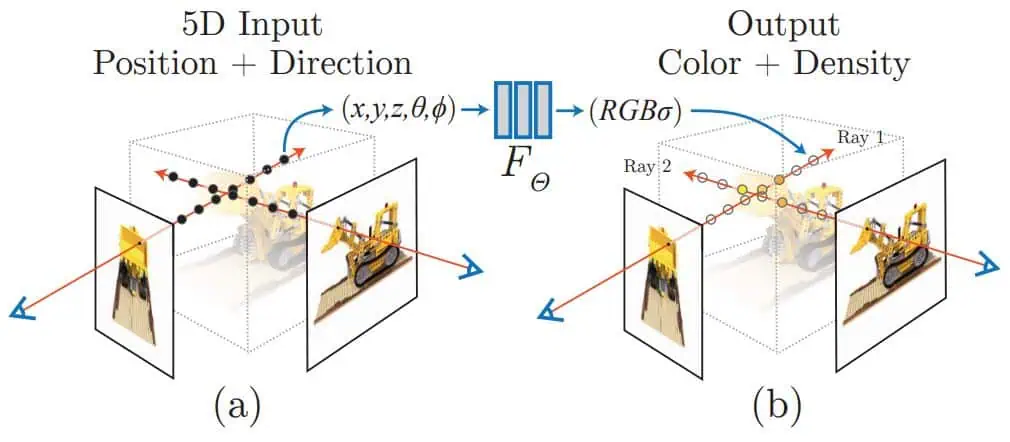
\includegraphics[width=1.0\linewidth]{res/02_literature/nerf.png}
    \end{center}
    \caption{NeRF ~\cite{mildenhall2020} work by sampling a 5D space and then compounding those approximations with corresponding transparency coefficients.}
    \label{fig:nerf}
\end{figure}

\subsection{Accelerating NeRF: Instant-NGP and Hybrid Representations}

Müller et al.~\cite{mller2022} addressed NeRF's high computational cost with Instant-NGP, a hybrid representation based on a multi-resolution hash encoding. The idea is to move the burden of representing high-frequency detail from the MLP to a learnable spatial data structure. A hierarchy of 3D hash tables stores per-voxel feature vectors at several resolutions. The MLP only needs to interpolate and decode these features rather than learning them from scratch. This cut training time from days to seconds without sacrificing visual quality, and it started a paradigm shift, the MLP became a decoder on top of an explicit spatial structure, not the primary container of geometry.

Instant-NGP spawned a small family of hybrid methods (DVGO, TensoRF, Plenoxels), all of which share the same architectural move, replace a purely implicit function with an explicit container of learnable parameters, and use the neural network only as a lightweight decoder. The outcome of the increasing reduction of the use of decoder culminates in the upcoming methods, where it is entirely removed.

\section{Explicit Radiance Fields: 3D Gaussian Splatting}

Kerbl et al.~\cite{kerbl2023} introduced a paradigm shift by removing the neural network (MLP) entirely from the radiance field equation. Instead of querying a black-box coordinate network, the scene is represented explicitly as an unstructured set of millions of 3D Gaussians. Each Gaussian carries a set of learned parameters: a 3D position, an opacity value, a 3D covariance matrix (stored efficiently as a scale and rotation vector), and view-dependent color. To handle complex lighting and specular reflections without heavy computation, this color is encoded using spherical-harmonic (SH) coefficients, allowing the splats to smoothly change appearance based on the camera angle. 

Rendering is handled not by computationally expensive volumetric ray-marching (which would be the obvious choice given that we are talking about actual 3D objects), but by \emph{splatting}. Each 3D Gaussian is mathematically projected onto the 2D image plane, and their resulting 2D projections are blended together in depth-sorted order via a tile-based rasterizer. Because this approach relies on the same fundamental projection and alpha-blending operations that GPU rasterization pipelines have been built around since the mid-1990s, the rendering process is radically faster than NeRF. The result is a system that, under the exact same training budget, matches or exceeds NeRF's visual fidelity while rendering at over $100$,FPS on standard consumer hardware. Perhaps equally important is the explicit nature of the representation: every single Gaussian has an interpretable spatial footprint. The entire optimized scene can be serialized as a standard, single PLY file, making it directly compatible with existing 3D software suites and incredibly easy to inspect visually. 

However, this explicit structure requires a more convoluted training procedure than continuous gradient descent on a compact MLP. As visualized in Figure~\ref{fig:gaussians-2}, the optimization involves a dynamic geometry-refinement process. The system periodically assesses the scene, executing adaptive densification to split or clone Gaussians in under-reconstructed regions, resetting opacity to prevent local minima, and pruning transparent or overly large splats. Despite its complexity, the numerical dynamics of this discrete structural optimization are well-understood, highly stable, and reproducible.

\begin{figure}[!ht]
    \begin{center}
    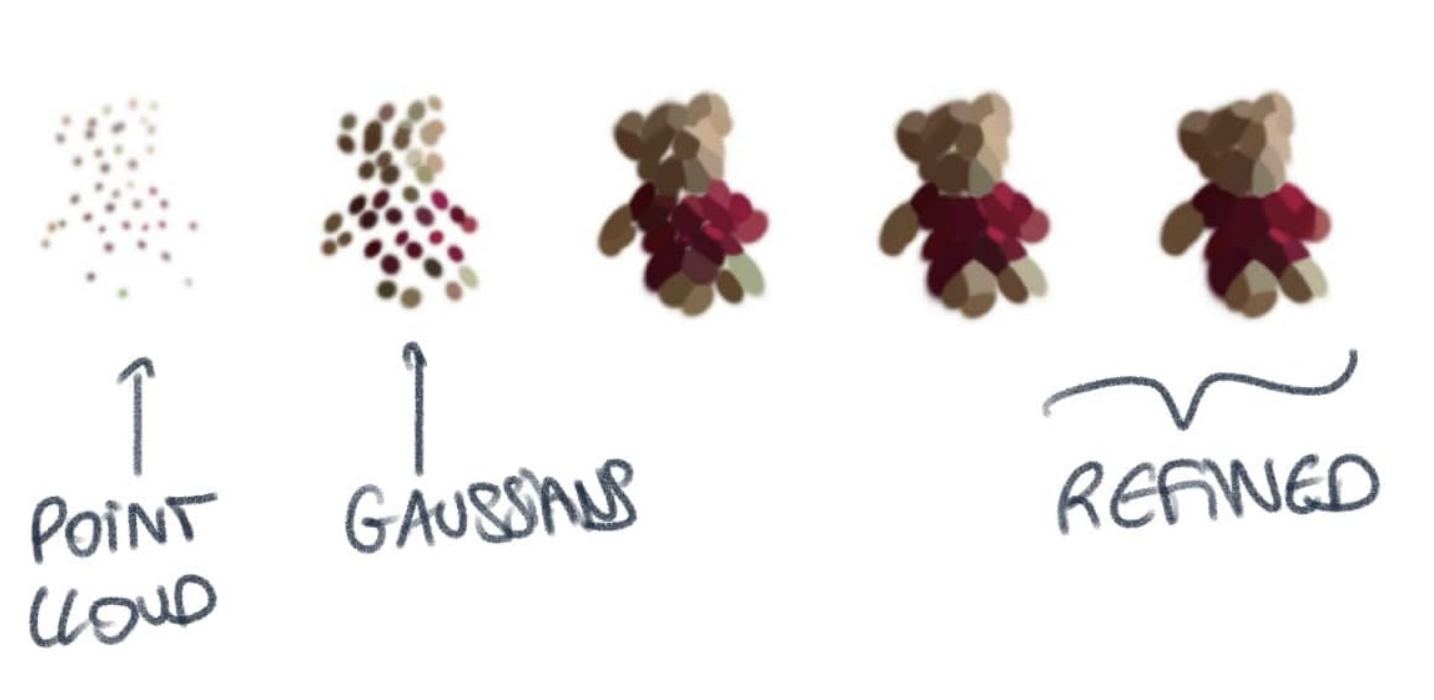
\includegraphics[width=0.9\linewidth]{res/02_literature/gaussian-1.png}
    \end{center}
    \caption{High-level visualization of how 3DGS takes sparse representation and refines it to better describe scene geometry. (\href{https://pyimagesearch.com/2024/12/09/3d-gaussian-splatting-vs-nerf-the-end-game-of-3d-reconstruction/}{graphic source})}
    \label{fig:gaussians-1}
\end{figure}

\newpage

Because of these massive advantages in speed and interpretability, 3DGS has rapidly become the foundational representation for dozens of derivative works. The research community has expanded it into mesh extraction (e.g., SuGaR, 2D Gaussian Splatting), storage compression (Scaffold-GS, Compact-3DGS), physically-based rendering for relighting (Relightable 3DGS), and, most relevant to this thesis, temporal extensions for dynamic scenes. Figure~\ref{fig:gaussians-2} illustrates the complete, end-to-end 3DGS pipeline that powers these advancements. The method relies on sparse point clouds generated by Structure-from-Motion (SfM) to initialize the Gaussians, providing a crucial structural foundation. It then enters an iterative optimization loop where the Gaussians are repeatedly rasterized into images, compared against ground-truth training views, and adjusted to minimize rendering error. The present work builds directly on this reference implementation of Kerbl et al., reusing its highly optimized differentiable rasterizer, its spherical-harmonic color parameterization, and its adaptive density control, ultimately extending this robust architecture with a novel temporal-tracking stage.

\begin{figure}[!ht]
    \begin{center}
    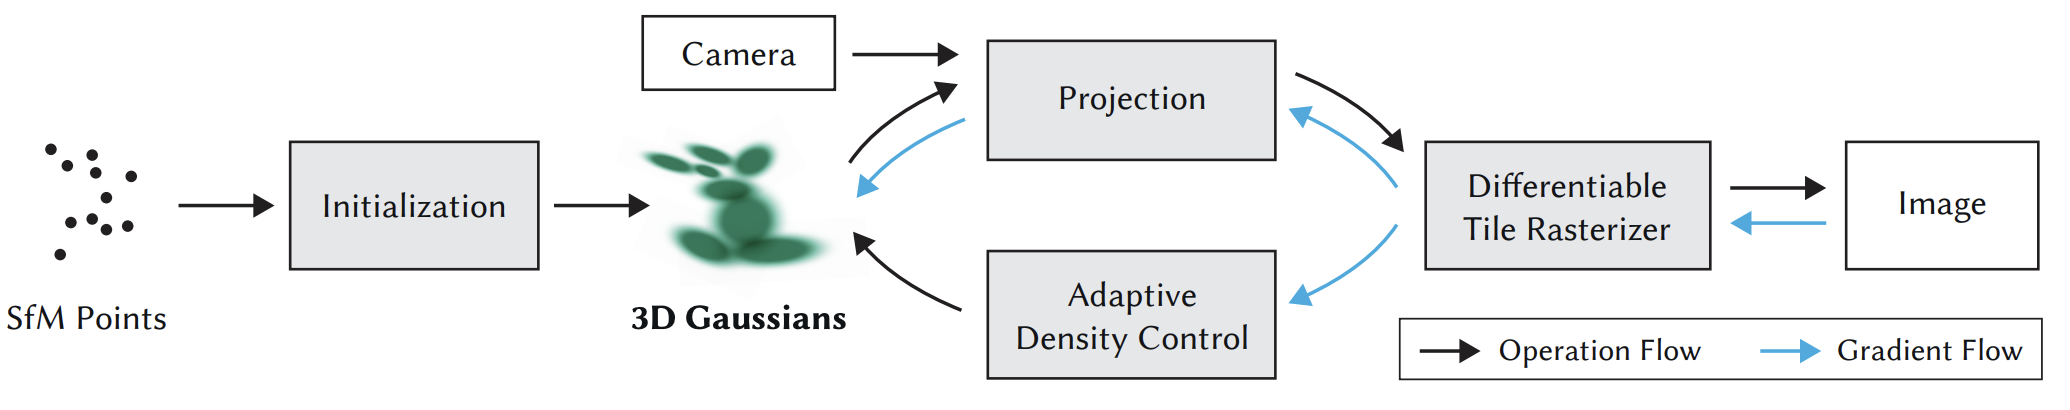
\includegraphics[width=0.9\linewidth]{res/02_literature/gaussian-2.png}
    \end{center}
    \caption{Visualization of entire 3DGS pipeline from the original paper ~\cite{kerbl2023}. The method takes in SfM points and perform a iterative optimization loop where gaussians are rasterized and adjusted to present views.}
    \label{fig:gaussians-2}
\end{figure}

\newpage

\section{Dynamic and Temporal Scene Representations}

Extending radiance fields to dynamic scenes is a substantially more recent idea than static reconstruction, and the literature on this topic is correspondingly less extensive. Existing methods fall broadly into three families, each of which inherits a different parent static method.

\subsection{Dynamic NeRF Variants}

The earliest family of dynamic neural-rendering methods extends NeRF with an auxiliary deformation field. D-NeRF \cite{pumarola2020} factorises the scene into a canonical radiance field $F_\theta^\text{canonical}$ and a time-conditioned deformation MLP $\Psi_\phi(\mathbf{x}, t)$:
\begin{equation}
    F_\theta^\text{dynamic}(\mathbf{x}, t, \mathbf{d}) = F_\theta^\text{canonical}\bigl(\mathbf{x} + \Psi_\phi(\mathbf{x}, t),\, \mathbf{d}\bigr).
\end{equation}
Nerfies \cite{park2021nerfies} refines this idea with a dedicated temporal regularisation to handle non-rigid human motion from a monocular camera. Both approaches share a common limitation: they inherit NeRF's per-ray cost, multiplied now by an additional MLP evaluation per sample, which makes the per-frame optimisation extremely slow. They are also structurally unsuitable for static-camera multi-view captures with long durations, since the deformation MLP must memorise the trajectory of every spatial location for the entire sequence.

\subsection{Dynamic Extensions of 3D Gaussian Splatting}

\noindent
Following the widespread adoption of 3DGS, three main temporal extensions have emerged. 

\paragraph{Deformable 3D Gaussians.} Yang et al.~\cite{yang2024deformable} mirror the D-NeRF recipe: a canonical Gaussian set $\mathcal{G}^\text{canonical}$ is augmented with a small deformation MLP $\Psi_\phi$ that, at every time $t$, outputs a per-Gaussian displacement of position, scale, and rotation:
\begin{equation}
    (\Delta \boldsymbol{\mu}_i, \Delta s_i, \Delta q_i) = \Psi_\phi(\boldsymbol{\mu}_i^\text{canonical}, t).
\end{equation}
The renderer then evaluates the standard 3DGS rasteriser on the deformed Gaussians. The approach preserves the rendering speed of 3DGS but introduces a dependence on the capacity of the deformation MLP, which must memorise the full motion of every physical feature in the scene. Training dynamics are also sensitive to the deformation MLP's positional encoding.

\paragraph{4D Gaussian Splatting.} Wu et al.~\cite{wu20244dgs} take a different route: they factorise the temporal variation of each Gaussian parameter into a product of spatial and temporal bases stored in a HexPlane-like structure, and decode the per-Gaussian deformation through a compact MLP. This factorisation is storage-efficient but imposes a low-rank assumption on the scene dynamics that is not always satisfied.

\paragraph{SpaceTime Gaussians.} Li et al.~\cite{li2024spacetime} replace the MLP-based temporal encoding with an explicit per-Gaussian polynomial. Each Gaussian carries its own low-degree polynomial coefficients for position, rotation, and opacity, which reduces inference cost at the price of an enlarged per-splat parameter set.

\subsection{Positioning of the Proposed Method}

The method developed in Chapter~3 sits in a deliberately minimalistic corner of this design space. Unlike Deformable 3DGS and 4D-GS, it uses \emph{no} auxiliary neural network or temporal basis. Unlike SpaceTime Gaussians, it does \emph{not} store per-Gaussian polynomial coefficients. Like Dynamic 3D Gaussians, it preserves the bijection between frame-0 and frame-$t$ Gaussians, but it does so without any explicit tracking loss, relying instead on a fixed topology, a first-order linear velocity prediction, and a hard freeze of the spherical-harmonic coefficients. The central claim of the thesis is that this ''less-is-more'' configuration is \emph{sufficient} for the characteristic regime of indoor multi-view video with static cameras, and empirically competitive with the more elaborate alternatives in that regime.

\section{Theoretical Background}

This section states the formal mathematical content of the two algorithms the thesis depends on: 
\begin{itemize}
    \item COLMAP's incremental Structure-from-Motion.
    
    \item Differentiable rasterisation pipeline of 3D Gaussian Splatting.
\end{itemize}

Chapter~3 builds on both without re-deriving them.

\subsection{Sparse Reconstruction via COLMAP}

COLMAP transforms an unordered set of input images $I = \{I_1, \dots, I_N\}$ into a sparse 3D point cloud and the associated camera poses. The pipeline proceeds in two phases.

\subsubsection{Correspondence search}

Feature extraction uses SIFT \cite{lowe1999sift}, which identifies scale- and rotation-invariant keypoints and assigns a $128$-dimensional descriptor to each. Pairwise feature matching produces correspondences. Matches are then geometrically verified through the epipolar constraint. A fundamental matrix $F$ (for uncalibrated cameras) or essential matrix $E$ (for calibrated cameras) is estimated with RANSAC, and matches $(x, x')$ satisfying
\begin{equation}
    x'^T F x = 0
\end{equation}
within a pixel tolerance are retained as inliers.

\subsubsection{Incremental reconstruction} 

The system is seeded with a two-view reconstruction obtained from an image pair with high inlier count and wide baseline. New images are registered by the Perspective-n-Point (PnP) algorithm, which solves for the pose $(R, t)$ that projects the already-triangulated 3D points onto the new image's 2D observations. As new images and points are added, mathematical drift accumulates and is periodically corrected by \emph{bundle adjustment}, a non-linear least-squares optimisation that jointly refines all 3D point positions and all camera parameters to minimise the total reprojection error:
\begin{equation}
    E = \sum_{i}\sum_{j} \rho\!\left(\left\| u_{ij} - \pi(K_i [R_i | t_i]\,X_j) \right\|_2^2\right),
\end{equation}
where $u_{ij}$ is the observed 2D location of 3D point $X_j$ in image $i$, $\pi$ is the pinhole projection function, $K_i$ the intrinsic matrix of camera $i$, and $\rho$ a robust loss (Huber or Cauchy) used to damp the influence of residual outliers. Bundle adjustment is the numerical backbone of modern SfM, without it, any incremental pipeline would accumulate unbounded drift over long trajectories.

\begin{figure}[!ht]
    \begin{center}
    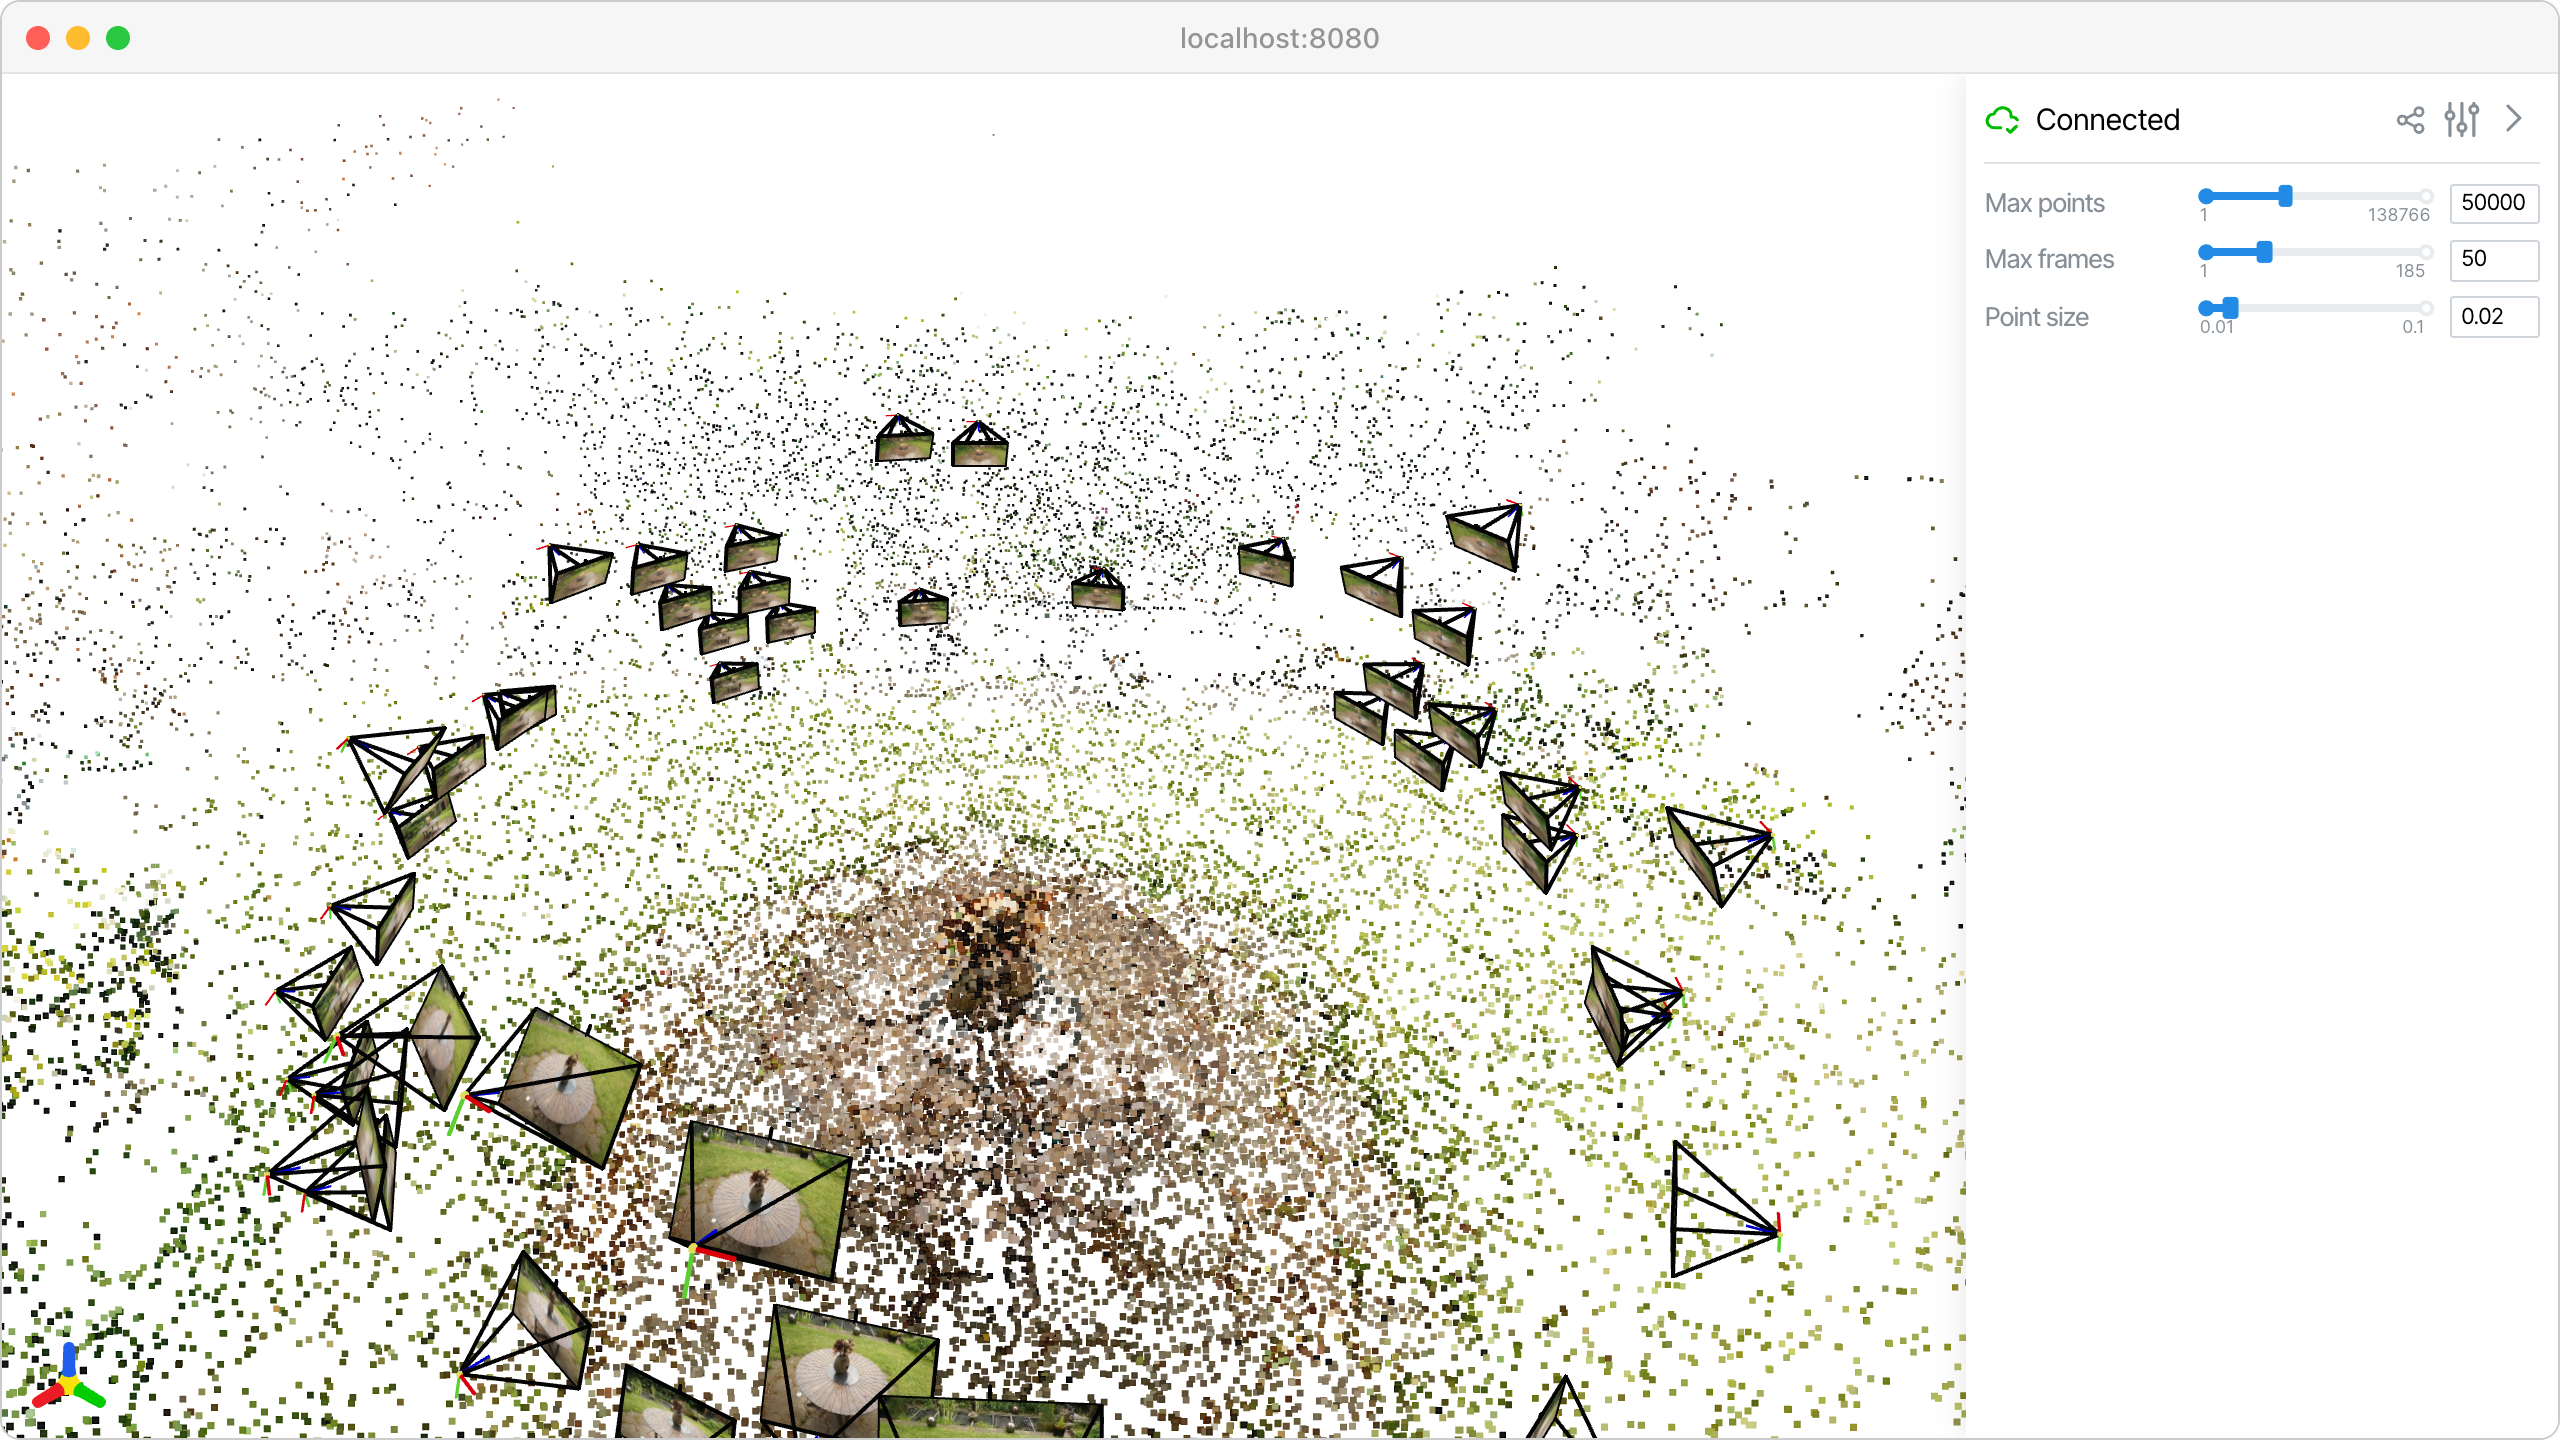
\includegraphics[width=0.9\linewidth]{res/02_literature/colmap-gui.png}
    \end{center}
    \caption{COLMAP's GUI after successful point cloud reconstruction. Views/cameras are represented as 3D pyramids floating in space. In the middle we can see a rough outline of an objected reconstructed using sparse colleciton of points.}
    \label{fig:colmap}
\end{figure}

\subsection{3D Gaussian Splatting}

3DGS represents a scene as a learnable point cloud of 3D Gaussians $\mathcal{G} = \{g_1, \dots, g_M\}$, where each primitive acts as a soft, semi-transparent ellipsoidal particle with learnable geometric and appearance parameters. The 3DGS framework can be divided into several steps that are presented in the following paragraphs.

\subsubsection{Volumetric Parameterisation} 

Each Gaussian is defined by a mean $\boldsymbol{\mu} \in \mathbb{R}^3$ and a 3D covariance matrix $\mathbf{\Sigma} \in \mathbb{R}^{3\times 3}$. Its contribution at a spatial location $\mathbf{x}$ is the unnormalised Gaussian:
\begin{equation}
    G(\mathbf{x}) = \exp\!\left(-\tfrac{1}{2} (\mathbf{x} - \boldsymbol{\mu})^T \mathbf{\Sigma}^{-1} (\mathbf{x} - \boldsymbol{\mu})\right).
\end{equation}
The covariance is not optimised directly. Instead, it is factorised into a rotation matrix $\mathbf{R}$ built from a unit quaternion $q \in \mathbb{R}^4$ and a diagonal scaling matrix $\mathbf{S}$ built from a log-scale vector $s \in \mathbb{R}^3$:
\begin{equation}
    \mathbf{\Sigma} = \mathbf{R}(q)\,\mathbf{S}(s)\,\mathbf{S}(s)^T \mathbf{R}(q)^T.
\end{equation}
This factorisation guarantees that $\mathbf{\Sigma}$ remains symmetric positive semi-definite for any $(q, s)$, so no projection step is needed during gradient descent.

Each Gaussian additionally carries a pre-activation opacity $\tilde{\sigma}$ (passed through a sigmoid at render time) and a view-dependent colour represented by spherical-harmonic coefficients up to degree $L = 3$. The view-dependent colour at a viewing direction $\mathbf{d} \in \mathbb{S}^2$ is:
\begin{equation}
    \mathbf{c}(\mathbf{d}) = \sum_{\ell = 0}^{L} \sum_{m=-\ell}^{\ell} \mathbf{k}_{\ell, m}\, Y_\ell^m(\mathbf{d}),
\end{equation}
where $Y_\ell^m$ is the real spherical-harmonic basis and $\mathbf{k}_{\ell, m} \in \mathbb{R}^3$ are the learnable coefficients. Storing only the DC coefficient is equivalent to a purely diffuse (Lambertian) material; higher-order coefficients capture view-dependent effects such as specularities.

\subsubsection{Projection and Differentiable Rasterisation.} 

Rendering projects each 3D Gaussian onto the image plane. Given a viewing transformation $\mathbf{W}$ and the Jacobian $\mathbf{J}$ of the local affine approximation of the projective transformation, the 2D projected covariance is:
\begin{equation}
    \mathbf{\Sigma}' = \mathbf{J}\,\mathbf{W}\,\mathbf{\Sigma}\,\mathbf{W}^T \mathbf{J}^T.
\end{equation}

The screen is divided into $N \times N$ pixel tiles. Gaussians are culled against the view frustum and depth-sorted tile-by-tile with a GPU radix sort. For every pixel, the final colour is the alpha-blend of the depth-sorted Gaussians overlapping that pixel:
\begin{equation}
    C = \sum_{i \in N} \mathbf{c}_i \alpha_i \prod_{j=1}^{i-1} (1 - \alpha_j), \qquad \alpha_i = \sigma_i \cdot G^{2D}(\mathbf{x}_\text{pixel}),
\end{equation}
where $G^{2D}$ is the projected 2D Gaussian evaluated at the pixel location and $\sigma_i$ is the Gaussian's opacity. This compositing rule is fully differentiable, gradients flow from the pixel colour back through the depth-sort, the 2D covariance, and ultimately to all optimisable parameters $(\boldsymbol{\mu}, q, s, \tilde{\sigma}, \{\mathbf{k}_{\ell, m}\})$.

\subsubsection{Adaptive Density Control} 

A critical feature of 3DGS is that the number of Gaussians is not fixed, it evolves during training through a cyclical process of densification and pruning driven by the accumulated view-space positional gradient $\|\nabla_{\boldsymbol{\mu}} \mathcal{L}\|_2$. The evolution strategy responds to two reconstruction errors, which visualizations can also be seen on Figure \ref{fig:gaussian3}:

\begin{itemize}
    \item \textbf{Under-reconstruction:} regions where Gaussians are too sparse. Diagnosed by high positional gradient \emph{combined with} small Gaussian scale, and resolved by \textbf{cloning}, i.e.\ duplicating the offending Gaussian and moving the clone along the gradient direction.
    \item \textbf{Over-reconstruction:} regions where a single large Gaussian attempts to cover complex geometry. Diagnosed by high positional gradient \emph{combined with} large Gaussian scale, and resolved by \textbf{splitting}, i.e.\ replacing the Gaussian with two children of reduced scale whose positions are sampled from the parent's 3D distribution.
\end{itemize}

In parallel, Gaussians whose opacity has decayed below a threshold are \textbf{pruned}, and every few thousand iterations all opacities are \textbf{reset} to a small ceiling to flush out semi-transparent ''floaters''. This entire machinery is active during the static reconstruction phase of the pipeline described in Chapter~3. Crucially, the dynamic extension proposed by this thesis \emph{disables} densification, pruning, and opacity reset after the first frame, freezing the topology of the Gaussian set so that per-primitive temporal correspondence is preserved across the entire video sequence. This design choice is motivated directly by the positioning discussed at the end of Section~2.4.

\begin{figure}[!ht]
    \begin{center}
    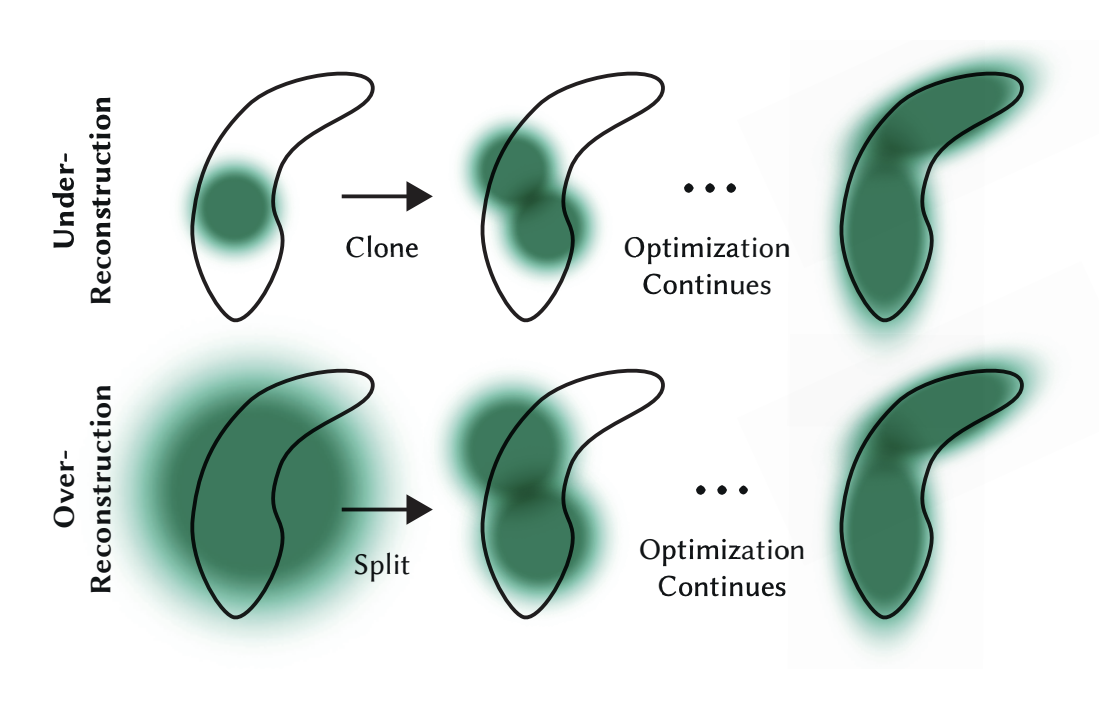
\includegraphics[width=0.9\linewidth]{res/02_literature/gaussian-3.png}
    \end{center}
    \caption{Visualizations present in the original paper \cite{kerbl2023} of how 3DGS solves the problem of under- and over-reconstruction.}
    \label{fig:gaussian3}
\end{figure}
